%=========================================================

% Here you can choose to compile with or without solutions.
% However, this definition is ignored if you use any
% command from the `Makefile`.
\providecommand{\withSol}{\iftrue}

%=========================================================

\documentclass
[twoside,english,colorbacktitle,accentcolor=tud9c]
{tudexercise}

\usepackage[T1]{fontenc}
\usepackage[latin9]{inputenc}
\usepackage{amstext}
\usepackage{amsmath}
\usepackage{graphicx}
\usepackage{setspace}
\usepackage{multicol}
\usepackage{mathtools}
\usepackage{dsfont}
\usepackage{units}
\usepackage{subfigure}
\usepackage{color}
\usepackage{booktabs}
\usepackage{fancyref}
\usepackage[ngerman,english]{babel}

%=========================================================

\def\homework{3}
\def\homeworkVer{1}
\def\homeworkSolVer{1}
\def\lecture{Robot Learning}
\def\semester{Winter Semester 2017/2018}
\def\prof{Prof. Dr. J. Peters, D. Tanneberg, M. Ewerton}
\def\deadline{Due date: Wednesday, 17 January 2018 (before the lecture)}

%=========================================================

\ifcsname withSol\endcsname\else
  \expandafter\let\csname withSol\expandafter\endcsname
                  \csname iffalse\endcsname
\fi

\withSol
	\usepackage[solutions]{iasHomework}
\else
	\usepackage{iasHomework}
\fi

%=========================================================

% USE YOUR NAMES!
\newcommand{\studentdata}{}
%\newcommand{\studentdata}{John Doe, 1234567 \qquad Jane Doe, 7654321}

\begin{document}
	
	\hwtitle{}
	\maketitle
	
	\begin{examheader}
		\normalsize
		\vspace{-1em}
		Name, Surname, ID Number \hfill \studentdata{}
		\vspace{-1em}
	\end{examheader} 
	
	\textbf{Name, Surname, ID Number \hfill \studentdata{}}
	
	\exercise{Optimal Control}
In this exercise, we consider a finite-horizon discrete time-varying Stochastic Linear Quadratic Regulator with Gaussian noise and time-varying quadratic reward function. Such system is defined as
%
\begin{align}
	\vec s_{t+1} = \mat A_t \vec s_t + \mat B_t a_t + \vec w_t\,, 
\end{align}
where $\vec s_t$ is the state, $a_t$ is the control signal, $\vec w_t \sim \gauss{\vec b_t}{\mat \Sigma_t}$ is Gaussian additive noise with mean $\vec b_t$ and covariance $\mat \Sigma_t$ and $t=0,1,\dots,T$ is the time horizon. 
The control signal $a_t$ is computed as
%
\begin{align}
	a_t = - \mat K_t \vec s_t + k_t
\end{align}
%
and the reward function is
%
\begin{align}
	reward_t = \begin{cases}
	- (\vec s_t - \vec r_t)\T \mat R_t (\vec s_t - \vec r_t) - a\T_t \mat H_t a_t  & \text{when \quad} t=0,1,\dots,T-1
	\\
	- (\vec s_t - \vec r_t)\T \mat R_t (\vec s_t - \vec r_t) & \text{when \quad} t=T
	\end{cases}
\end{align}
	
\textbf{Note: the notation used in Marc Toussaint's notes ``\textit{(Stochastic) Optimal Control''} is different from the one used in the lecture's slides.}	
	
\begin{questions}

%----------------------------------------------

\begin{question}{Implementation}{8}
	Implement the LQR with the following properties
	\begin{align*}
	\vec s_0 & \sim \gauss{\vec 0}{\mat I} &	T &= 50
	\\
	\mat A_t &= \begin{bmatrix}
       1 & 0.1\\
       0 & 1
    \end{bmatrix} &
	\mat B_t &= \begin{bmatrix}
       0 \\
       0.1
    \end{bmatrix}
    \\
	\vec b_t &= \begin{bmatrix}
       5\\
       0
    \end{bmatrix} & \mat \Sigma_t &= \begin{bmatrix}
       0.01 & 0\\
       0 & 0.01
    \end{bmatrix}
	\\
	\mat K_t &= \begin{bmatrix}
       5 &
       0.3
    \end{bmatrix} & 
	k_t &= 0.3 & 
	\\
	\mat H_t &= 1 & 		
	\mat R_t &= \begin{cases}
	\begin{bmatrix}
	100000 &0\\
	0&0.1
	\end{bmatrix}  & \text{if \quad $t=14$ or 40}
	\\
	\begin{bmatrix}
	0.01 &0\\
	0&0.1
	\end{bmatrix} & \text{otherwise}
	\end{cases}	
	&
	\vec r_t &= \begin{cases}
	\begin{bmatrix}
	10\\
	0
	\end{bmatrix}  & \text{if \quad} t=0,1,\ldots,14
	\\
	\begin{bmatrix}
	20\\
	0
	\end{bmatrix}  & \text{if \quad} t=15,16,\ldots,T
	\end{cases}	
	\end{align*}
	
	Execute the system 20 times.
	Plot the mean and 95\% confidence (see ``68--95--99.7 rule'' and matplotlib.pyplot.fill\_between function) over the different experiments of the state $\vec s_t$ and of the control signal $\vec a_t$ over time. 
	How does the system behave? 
	Compute and write down the mean and the standard deviation of the cumulative reward over the experiments. 
	Attach a snippet of your code.
	
\begin{answer}
	
\begin{center}
	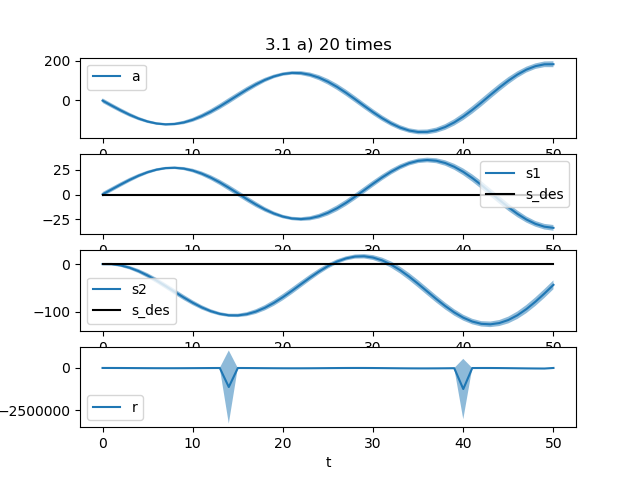
\includegraphics[width=0.75\textwidth]{img/1a_20.png}
	\captionof{figure}{States and action of an instable controller. Mean and 95 \% confidence level.}
\end{center}

The system is instable cause the eigenvalues of the discrete system ( derived from the A-BK matrix) are: $\lambda_i = 0.985 \pm i 0.2231 i$. The eigenvalues are outside the unit circle. For this reason the system is instable and  oscillates (see state s1, s2 ).

The mean of the  cummulative reward over the experiments:  $\sum rw = -2717991.1$

The standard deviation of the cummulative reward is: 681486

\lstinputlisting[caption=Code too calc the states and actions]{code/a1_a.py}
\end{answer}

\end{question}

%---------------------------------

\begin{question}{LQR as a P controller}{4}

	The LQR can also be seen as a simple P controller of the form
	%
	\begin{align}
		a_t = \mat K_t (\vec s^\text{des}_t - \vec s_t) + k_t\,,
	\end{align}
	%
	which corresponds to the controller used in the canonical LQR system with the introduction of the target $\vec s^\text{des}_t$.
	
	Assume as target 
	\begin{align}
        \vec s^\text{des}_t = \vec r_t = \begin{cases}
        \begin{bmatrix}
        10\\
        0
        \end{bmatrix}  & \text{if \quad} t=0,1,\ldots,14
        \\
        \begin{bmatrix}
        20\\
        0
        \end{bmatrix}  & \text{if \quad} t=15,16,\ldots,T
        \end{cases}	
	\end{align}
    
    Use the same LQR system as in the previous exercise and run 20 experiments. Plot in one figure the mean and 95\% confidence (see ``68--95--99.7 rule'' and matplotlib.pyplot.fill\_between function) of the first dimension of the state, for both $\vec s^\text{des}_t = \vec r_t$ and $\vec s^\text{des}_t = \vec 0$.
\end{question}

\begin{answer}
\begin{center}
	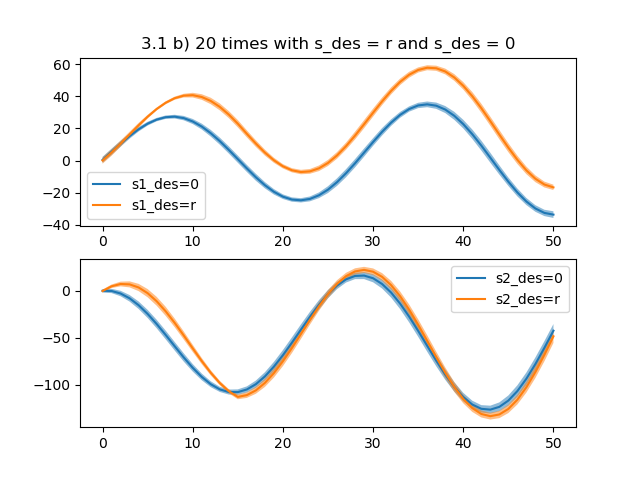
\includegraphics[width=0.75\textwidth]{img/1b_20.png}
	\captionof{figure}{States of an instable controller. Mean and 95 \% confidence level. Once with s\_des=0 and once with s\_des=r.}
\end{center}

Since t=40 the state s1\_des=r oscillates around 20. Whereas the state s1\_des = 0 oscillates a little bit lower.
	
\end{answer}


%---------------------------------
	
	
\begin{question}{Optimal LQR}{8}
	To compute the optimal gains $\mat K_t$ and $\vec k_t$, which maximize the cumulative reward, we can use an analytic optimal solution. This controller recursively computes the optimal action by
	\begin{align}
		a_t^* &= -(\mat H_t + \mat B^T_t \mat V_{t+1}\mat B_t)^{-1}	\mat B^T_t (\mat V_{t+1} (\mat A_t \vec s_t+\mat b_t )- \vec v_{t+1} ),
	\end{align}
	which can be decomposed into
	\begin{align}
		\mat K_t &= -(\mat H_t + \mat B^T_t \mat V_{t+1}\mat B_t)^{-1}	\mat B^T_t \mat V_{t+1} \mat A_t,
		\\
		\mat k_t &= -(\mat H_t + \mat B^T_t \mat V_{t+1}\mat B_t)^{-1}	\mat B^T_t (\mat V_{t+1} \mat b_t - \vec v_{t+1}).
	\end{align}
	%
	where
	%
	\begin{align}
		\mat M_t &= \mat B_t(\mat H_t + \mat B^T_t \mat V_{t+1}\mat B_t)^{-1}	\mat B^T_t \mat V_{t+1} \mat A_t
		\\
		\mat V_t &=
		\begin{cases}
	       \mat R_t + (\mat A_t - \mat M_t)^T\mat V_{t+1}\mat A_t & \text{when \quad} t = 1...T-1
	       \\
	       \mat R_t & \text{when \quad} t = T
	    \end{cases}
	    \\
		\mat v_t &= 
		\begin{cases}
	       \mat R_t\vec r_t + (\mat A_t - \mat M_t)^T(\vec v_{t+1} - \mat V_{t+1}\mat b_t) & \text{when \quad} t = 1...T-1
	       \\
	       \mat R_t\vec r_t & \text{when \quad} t = T
	    \end{cases}
	\end{align}		 

	Run 20 experiments with $\vec s^\text{des}_t = \vec 0$ computing the optimal gains $\mat K_t$ and $\vec k_t$. Plot the mean and 95\% confidence (see ``68--95--99.7 rule'' and matplotlib.pyplot.fill\_between function) of both states for all three different controllers used so far. Use one figure per state. 
	Report the mean and std of the cumulative reward for each controller and comment the results. Attach a snippet of your code.

\begin{answer}
	\begin{center}
		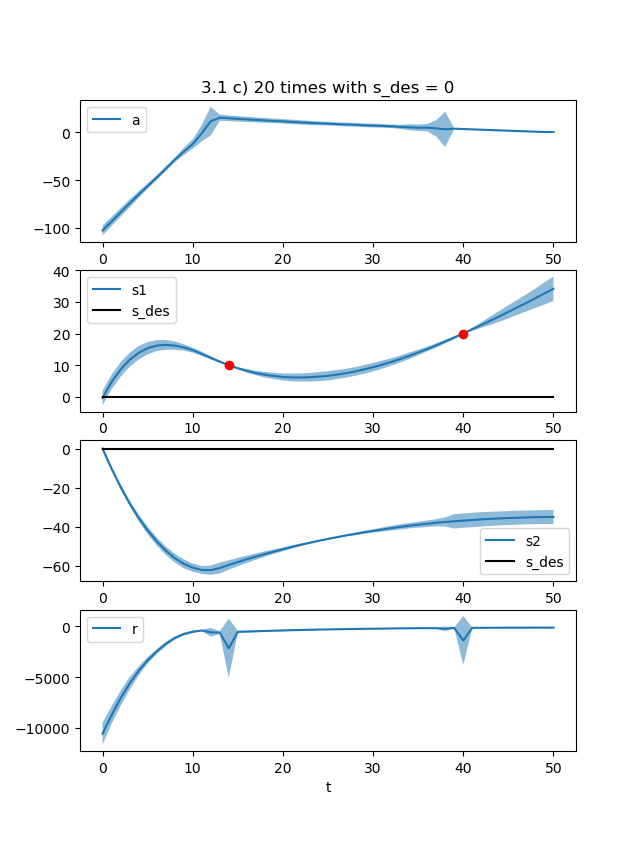
\includegraphics[width=0.75\textwidth]{img/1c_1.png}
		\captionof{figure}{Action, states and reward of the optimal controller.}
	\end{center}

	\begin{center}
		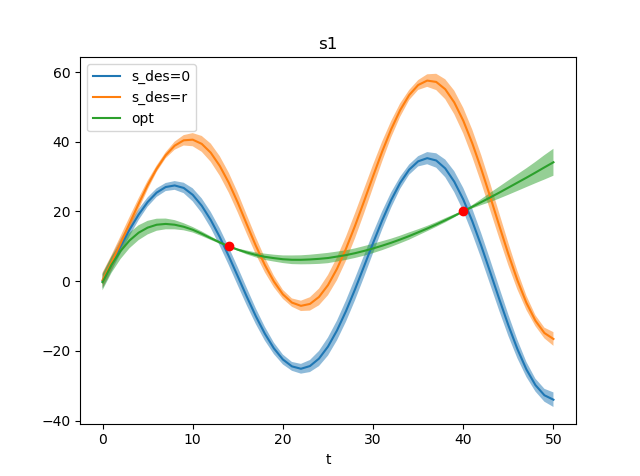
\includegraphics[width=0.75\textwidth]{img/1c_2.png}
		\captionof{figure}{State 1 of all three controllers compared.}
	\end{center}

	\begin{center}
		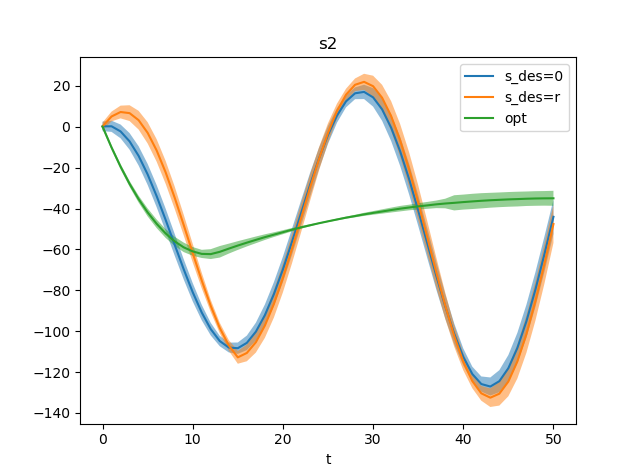
\includegraphics[width=0.75\textwidth]{img/1c_3.png}
		\captionof{figure}{State 2 of all three controllers compared.}
	\end{center}

	\begin{center}
		\begin{tabular}{|l|r|r|}
			\hline 
			cumulative reward & mean & std \\ 
			\hline 
			s\_des = 0 & -2739815.9 & 424072.8 \\ 
			\hline 
			s\_des = r & -105631266.4 & 11544950.4 \\ 
			\hline 
			opt & -61296.8 & 3966.4 \\ 
			\hline 
		\end{tabular}
		\captionof{table}{Rewards of the diffeerent controller}
	\end{center}	

	The only important part of the reward is the first state at t=14 and t=40. There R equals 100000 and because of this these timesteps have a much higher weight in the cumulative reward. All other timesteps have a R smaller 1 and a really small weight. State 2 has a small R at every timestep, so it is not important for the cumulative reward. 
	
	The desired state value is described by r. It equals 10 at t=14 and 20 at t=40. So the trajectory should go through this points (marked with red dots) to minimize the reward.

	The optimal controller meats this requirement, like you can see in the plot. The first controller is unstable and oscillates, but its trajectory also is near to the desired points. The second trajectory is also unstable and it is far away from the desired points. Because of this, the second trajectory has a really high negative reward. The first controller has a much smaller negative reward, but it also is very high. The optimal controller has a really small negative reward, compared too the two other controllers.
	\lstinputlisting[caption=code too calc the optimal controller]{code/a1_c.py}
\end{answer}
\end{question}

%----------------------------------------------

\end{questions}

	
	
\newif\ifvimbug
\vimbugfalse

\ifvimbug
\begin{document}
\fi

\exercise{Reinforcement Learning}

You recently acquired a robot for cleaning you apartment but you are not happy with its performance and you decide to reprogram it using the latest AI algorithms. As a consequence the robot became self-aware and, whenever you are away, it prefers to play with toys rather than cleaning the apartment. Only the cat has noticed the strange behavior and attacks the robot. The robot is about to start its day and its current perception of the environment is as following 
%
\begin{center}
	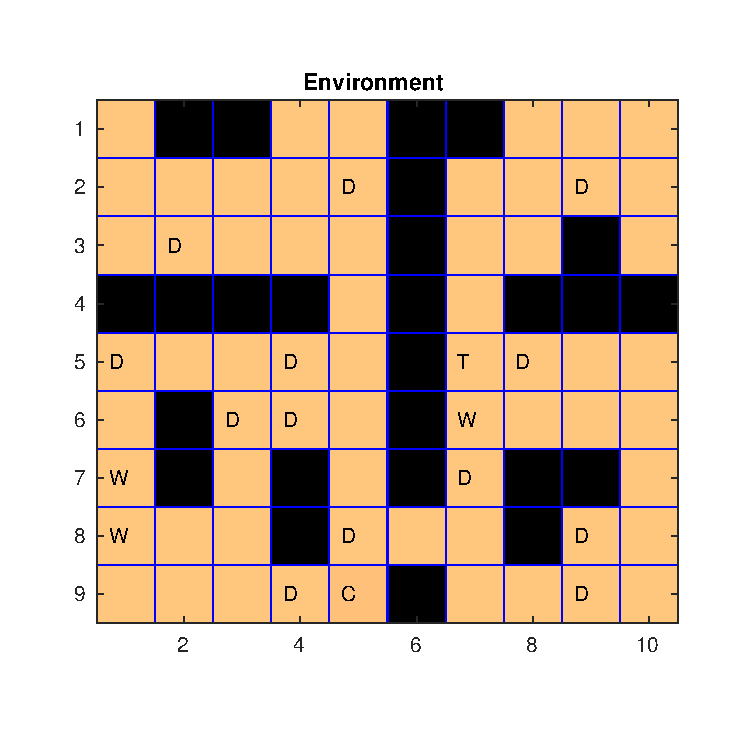
\includegraphics[width=0.75\textwidth]{gridworld.pdf}
\end{center}
%
The black squares denote extremely dangerous states that the robot must avoid to protect its valuable sensors. The reward of such states is set to $r_\textrm{danger}=-10^5$ (NB: the robot can still go through these states!). Moreover, despite being waterproof, the robot developed a phobia of water (W), imitating the cat. The reward of states with water is $r_\textrm{water}=-100$. The robot is also afraid of the cat (C) and tries to avoid it at any cost. The reward when encountering the cat is $r_\textrm{cat}=-3000$. The state containing the toy (T) has a reward of $r_\textrm{toy}=1000$, as the robot enjoys playing with them. Some of the initial specification still remain, therefore the robot receives $r_\textrm{dirt}=35$ in states with dirt (D).

State rewards can be collected at every time the robot is at that state. 
The robot can perform the following actions: \textit{down, right, up, left} and
\textit{stay}.

In our system we represent the actions with the an ID (0, 1, 2, 3, 4), while the grid is indexed as $\{ \texttt{row}, \texttt{column} \}$. The robot can't leave the grid as it is surrounded with walls.
A skeleton of the gridworld code and some plotting functions are available at the webpage.
For all the following questions, always attach a snippet of your code.


\begin{questions}

\begin{question}{Finite Horizon Problem}{14}
In the first exercise we consider the finite horizon problem, with horizon $T=15$ steps.
The goal of the robot is to maximize the expected return 
\begin{equation}
J_\pi = \mathbb{E}_\pi\left[\sum_{t=1}^{T-1}r_t(s_t,a_t)+r_T(s_T)\right], \label{Eq:J}
\end{equation}
according to policy $\pi$, state $s$, action $a$, reward $r$, and horizon $T$. Since rewards in our case are independent of the action and the actions are deterministic, Equation~\eqref{Eq:J} becomes
\begin{equation}
J_\pi = \sum_{t=1}^{T}r_t(s_t).
\end{equation}
Using the Value Iteration algorithm, determine the optimal action for each state when the robot has 15 steps left. Attach the plot of the policy to your answer and a mesh plot for the value function. Describe and comment the policy: is the robot avoiding the cat and the water? Is it collecting dirt and playing with the toy? With what time horizon would the robot act differently in state $(9,4)$?

\begin{answer}
	

\noindent\begin{minipage}{.5\textwidth}
	\centering
	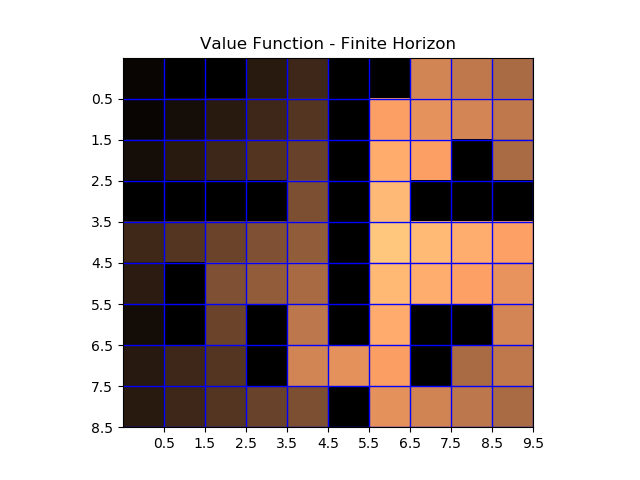
\includegraphics[width=1\textwidth]{img/value_2a.png} 
	\captionof{figure}{T=15, finite horizon Value Function}
	\label{fig:2a1}            
\end{minipage}%
\begin{minipage}{.5\textwidth}
	\centering
	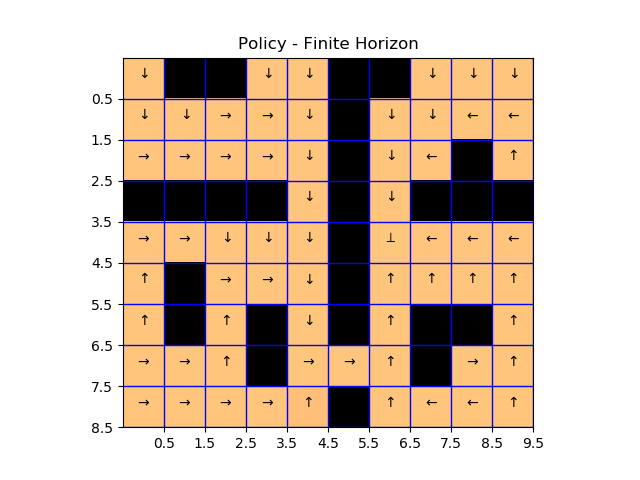
\includegraphics[width=1\textwidth]{img/policy_2a.png} 
	\captionof{figure}{T=15, finite horizon Policy}
	\label{fig:2a2}               
\end{minipage}
\begin{minipage}{.5\textwidth}
	\centering
	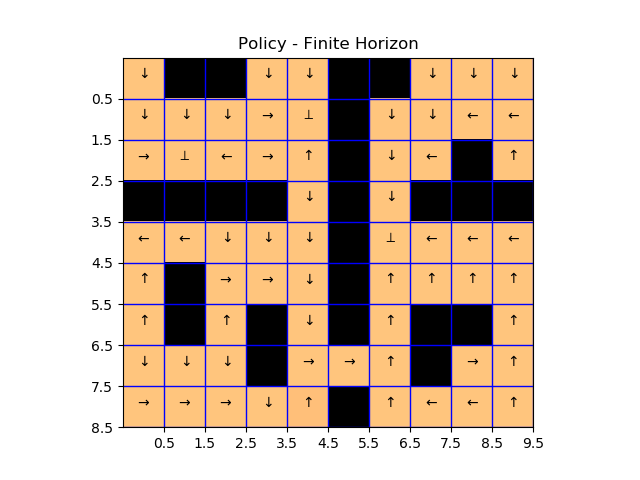
\includegraphics[width=1\textwidth]{img/2a_T10.png} 
	\captionof{figure}{T=10, finite horizon Policy}
	\label{fig:2a3}               
\end{minipage}

Policy of the robot:\\
The robot is trying to avoid the water and the cat(for T=15) if possible (see for example state(8,1) the robot is not moving to state 7,1 as this state is punished cause of its water). The robot is moving from all start states to the max. reward position (the toy at 5,7) avoiding all dangerous states. Thereby the robots is not so afraid of small punishments by the cat or water and moves also over these fields in order to reach the toy!

For T=10 the robot is moving differently and trying to avoid to move over the Cat's state at 9,4 (see Figure \ref{fig:2a3}).
	
\end{answer}

\end{question}

%----------------------------------------------


\begin{question}{Infinite Horizon Problem - Part 1}{4}
We now consider the infinite horizon problem, where $T=\infty$. Rewrite Equation~\eqref{Eq:J} for the infinite horizon case adding a discount factor $\gamma$. Explain briefly why the discount factor is needed.

\begin{answer}
Theory: \\
In the infinite time horizon case (when you live forever), the time index is not part of the state.  The optimal policy is time-independent: $\pi_t^*(a|s)=\pi^*(a|s)$. The reward and the transition model can no longer be time-dependent. There is a single stationary value function for all times. There are two different approaches to learning:
\begin{itemize}
	\item Value Iteration: Same as before just choose a large T for which the value function converges
	\item Policy Iteration: Learn a value function for the current policy. Update this policy and learn a new value function. Repeat.
\end{itemize}
Optimal policy for infinite horizon: $\pi^*=argmax_\pi J_\pi, \quad J_\pi=\sum_{t=0}^\infty \gamma^t r(s_t, a_t)$

In this case here:\\
\begin{equation}
J_\pi = \sum_{t=1}^{\infty} \gamma^t r_t(s_t).
\end{equation}

The discount factor $0<=\gamma<1$ trades-off long term vs. immediate reward. Without a discount factor many or all policies have infinite expected reward. For this reason a discount factor is required. Thereby future rewards $r_t(s,a)$ are discounted by $\gamma$ per time step.

	
\end{answer}

\end{question}

%----------------------------------------------


\begin{question}{Infinite Horizon Problem - Part 2}{6}
Calculate the optimal actions with the infinite horizon formulation. Use a discount factor of $\gamma=0.8$ and attach the new policy and value function plots.
What can we say about the new policy? Is it different from the finite horizon scenario? Why?

\begin{answer}
\noindent\begin{minipage}{.5\textwidth}
	\centering
	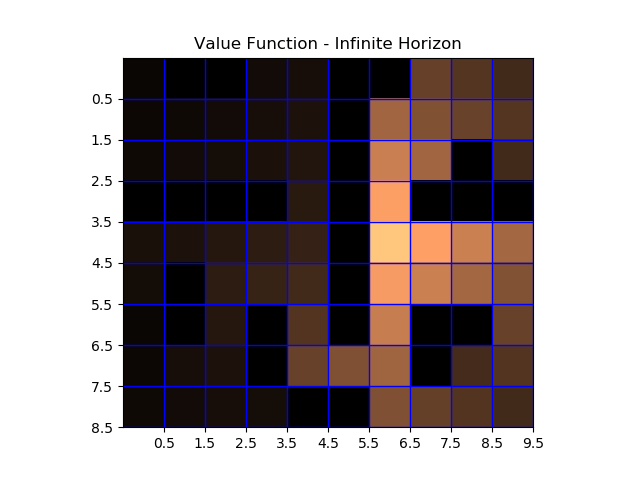
\includegraphics[width=1\textwidth]{img/infinitehorizon_2c.png} 
	\captionof{figure}{T=100, gamma=0.8 infinite horizon Value Function}
	\label{fig:2c1}            
\end{minipage}%
\begin{minipage}{.5\textwidth}
	\centering
	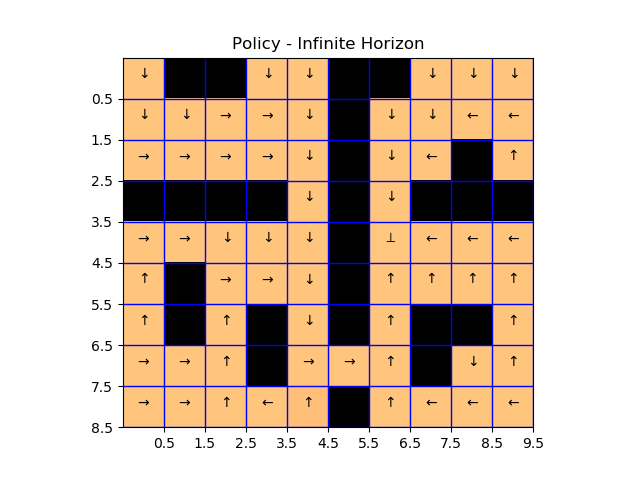
\includegraphics[width=1\textwidth]{img/policy_2c.png} 
	\captionof{figure}{T=100, gamma=0.8, infinite horizon Policy}
	\label{fig:2c2}               
\end{minipage}
\end{answer}

If the robot lives forever it avoids the cat to reach the toy! This is the only huge difference compared to the finite horizon scenario.

\end{question}

%----------------------------------------------


\begin{question}{Finite Horizon Problem with Probabilistic Transition Function}{10}
After a fight with the cat, the robot experiences control problems. 
For each of the actions \textit{up, left, down, right}, the robot has now a probability $0.7$ of correctly performing it and a probability of $0.1$ of performing another action according to the following rule: if the action is \textit{left} or \textit{right}, the robot could perform \textit{up} or \textit{down}. If the action is \textit{up} or \textit{down}, the robot could perform \textit{left} or \textit{right}.
Additionally, the action can fail causing the robot to remain on the same state with probability $0.1$.
Using the finite horizon formulation, calculate the optimal policy and the value function. Use a time horizon of $T=15$ steps as before. Attach your plots and comment them: what is the most common action and why does the learned policy select it?

\begin{answer}
	\begin{answer}
		\noindent\begin{minipage}{.5\textwidth}
			\centering
			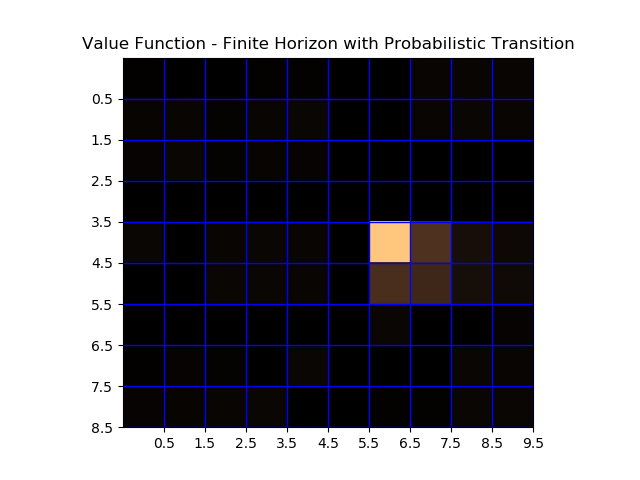
\includegraphics[width=1\textwidth]{img/value_2d.png} 
			\captionof{figure}{T=15, finite horizon Value Function}
			\label{fig:2d1}            
		\end{minipage}%
		\begin{minipage}{.5\textwidth}
			\centering
			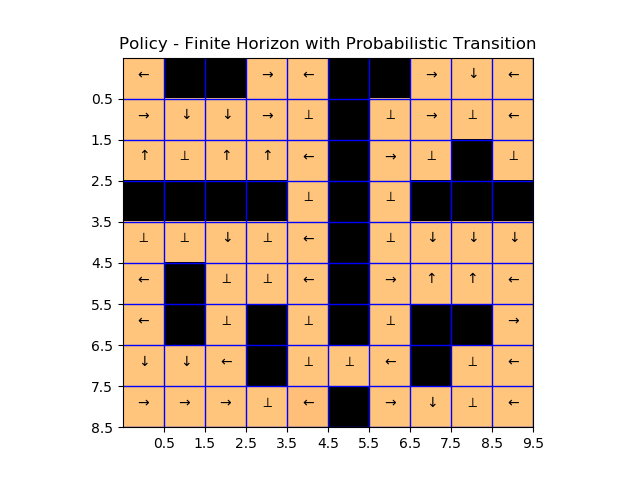
\includegraphics[width=1\textwidth]{img/policy_2d.png} 
			\captionof{figure}{T=15, finite horizon Policy}
			\label{fig:2d2}               
		\end{minipage}
	\end{answer}
	
\end{answer}

One of the more common action's is to stay at a reward position not risking a wrong movement to a punished position. One example is the state at 9,4. At this position the robot does not risk to move wrong in the right direction (into the cat). The learned policy rather let's the robot wait at a certain position than risking to move wrong into a punished state. One reason for that is the quite high probability of moving wrong (0.1).

\end{question}

%----------------------------------------------


\begin{question}[bonus]{Reinforcement Learning - Other Approaches}{8}
What are the two assumptions that let us use the Value Iteration algorithm? What if they would have been not satisfied? Which other algorithm would you have used? Explain it with your own words and write down its fundamental equation.

\begin{answer}
Assumptions: agent gets to observe the state 	
	
\end{answer}
\end{question}


\end{questions}

	
\end{document}
